\chapter{TRIỂN KHAI ỨNG DỤNG}

thanh toán hiển thị nút “Đã thanh toán” màu xanh ở trạng thái disabled, không cho phép thao tác thêm.

Hình 3.10 Giao diện Quản lý phí phạt – duyệt và theo dõi các khoản phí phát sinh

Như vậy, Librarian UI không chỉ đơn thuần là một giao diện hiển thị dữ liệu mà còn là một ứng dụng quản lý nghiệp vụ hoàn chỉnh, đáp ứng đầy đủ quy trình làm việc hàng ngày của Thủ thư. Việc tách biệt hoàn toàn giữa Reader UI và Librarian UI không chỉ giúp mỗi giao diện tập trung vào đúng đối tượng người dùng của mình, mà còn thể hiện nguyên tắc phân chia trách nhiệm (Separation of Concerns) trong thiết kế phần mềm. Mỗi giao diện có thể được phát triển, kiểm thử và triển khai độc lập, phù hợp với mô hình microservices mà toàn bộ hệ thống đang theo đuổi.

\section{Thử nghiệm thay đổi tham số}

\section{Thử nghiệm thay đổi tham số}

\subsection{Thay đổi chính sách mượn sách}

Một trong những yêu cầu quan trọng của hệ thống quản lý thư viện là khả năng điều chỉnh linh hoạt các tham số vận hành mà không cần sửa đổi mã nguồn. Dịch vụ N2 hỗ trợ điều này thông qua các API cấu hình chính sách (policy API) và cơ chế lưu trữ tham số trong cơ sở dữ liệu. Tham số giới hạn mượn hàng tháng (MonthlyBorrowLimit): Tham số này quy định số lượng sách tối đa mà một độc giả có thể giữ cùng lúc (bao gồm cả sách đang mượn và đang chờ duyệt). Giá trị mặc định là 5 cuốn. Thủ thư có thể thay đổi tham số này qua API:

PUT /api/circulation/settings/prices \{ "monthlyBorrowLimit": 3 \}

Khi tham số được thay đổi, N2 ghi nhận vào cơ sở dữ liệu và phát sự kiện BorrowPolicyUpdated để các dịch vụ khác có thể cập nhật logic hiển thị trên giao diện. Việc giảm giới hạn từ 5 xuống 3 sẽ ngay lập tức ảnh hưởng đến các yêu cầu mượn mới: độc giả đang giữ 3-4 cuốn sẽ bị từ chối khi cố mượn thêm. Thử nghiệm: Nhóm em đã tiến hành thay đổi MonthlyBorrowLimit từ 5 xuống 2 và kiểm tra trên Reader UI. Kết quả cho thấy khi một độc giả đang có 2 cuốn sách (1 đang mượn, 1 chờ duyệt), hệ thống từ chối yêu cầu mượn thêm với thông báo: “Bạn đã đạt giới hạn mượn. Mỗi độc giả chỉ được giữ tối đa 2 cuốn đang mượn hoặc chờ xử lý.” Khi tăng giới hạn trở lại 5, độc giả có thể tiếp tục mượn bình thường.

\subsection{Thay đổi chính sách phí phạt}

Hệ thống phí phạt của N2 được thiết kế với năm tham số có thể cấu hình độc lập, cho phép thư viện điều chỉnh chính sách phí phù hợp với từng giai đoạn hoặc đối tượng độc giả. Các tham số phí:

• BorrowPricePerBook – Phí mượn mỗi cuốn sách (mặc định: 5.000 VNĐ)

• DailyOverdueFine – Phí quá hạn mỗi ngày (mặc định: 5.000 VNĐ/ngày)

• LightDamageFine – Phí hư hỏng nhẹ (mặc định: 20.000 VNĐ)

• HeavyDamageFine – Phí hư hỏng nặng (mặc định: 100.000 VNĐ)

• LostFine – Phí mất sách (mặc định: 100.000 VNĐ)

Tất cả các tham số được cập nhật đồng thời qua một API duy nhất:

PUT /api/circulation/settings/prices \{ "borrowPricePerBook": 10000, "dailyOverdueFine": 5000, "lightDamageFine": 30000,

\section{Lược đồ cơ sở dữ liệu (ERD)}

\section{Lược đồ cơ sở dữ liệu (ERD)}

Cơ sở dữ liệu CirculationDB được thiết kế theo nguyên tắc Database per Service trong kiến trúc microservices, chỉ chứa các bảng phục vụ riêng cho nghiệp vụ lưu thông. Dữ liệu về sách và người dùng được lấy từ N1 và N3 thông qua API, N2 chỉ lưu các reference ID để liên kết.

BorrowTransactions FineCharges PK Id, BookId, UserId N:1 PK Id, FK TransId

BorrowedAt, DueAt, Status Amount, Reason, Status

Reference N:1

Books (cache) RevenueRecords PublishedEventLogs PK BookId, TenSach PK Id, FK RefId PK Id, Source

TacGia, SoLuong SourceType, Amount EventType, Payload

Users (cache) ReaderFavorites PK Id, Username PK Id, UserKey, BookId

Role, CardNumber TenSach, TacGia

Hình 3.12 Lược đồ cơ sở dữ liệu CirculationDB

Bảng 3.1 Mô tả chi tiết các bảng trong CirculationDB

Bảng Khóa chính Số cột Mô tả BorrowTransactions Id (GUID) 10 Phiếu mượn/trả sách, lưu toàn bộ lịch sử giao dịch FineCharges Id (GUID) 8 Phí phạt phát sinh khi trả quá hạn, hư hỏng, mất sách RevenueRecords Id (GUID) 7 Doanh thu từ phí mượn sách và thanh toán phí phạt PublishedEventLogs Id (GUID) 6 Nhật ký sự kiện phục vụ đồng bộ trạng thái liên service Users Id (GUID) 9 Cache thông tin người dùng từ N3 để tra cứu nhanh Books Id (int) 5 Cache thông tin sách từ N1 để giảm gọi API ReaderFavorites Id (GUID) 11 Danh sách sách yêu thích của độc giả

\clearpage
\section*{H?nh ?nh v? s? ?? minh h?a}
\addcontentsline{toc}{section}{H?nh ?nh v? s? ?? minh h?a}
\begin{figure}[H]
\centering
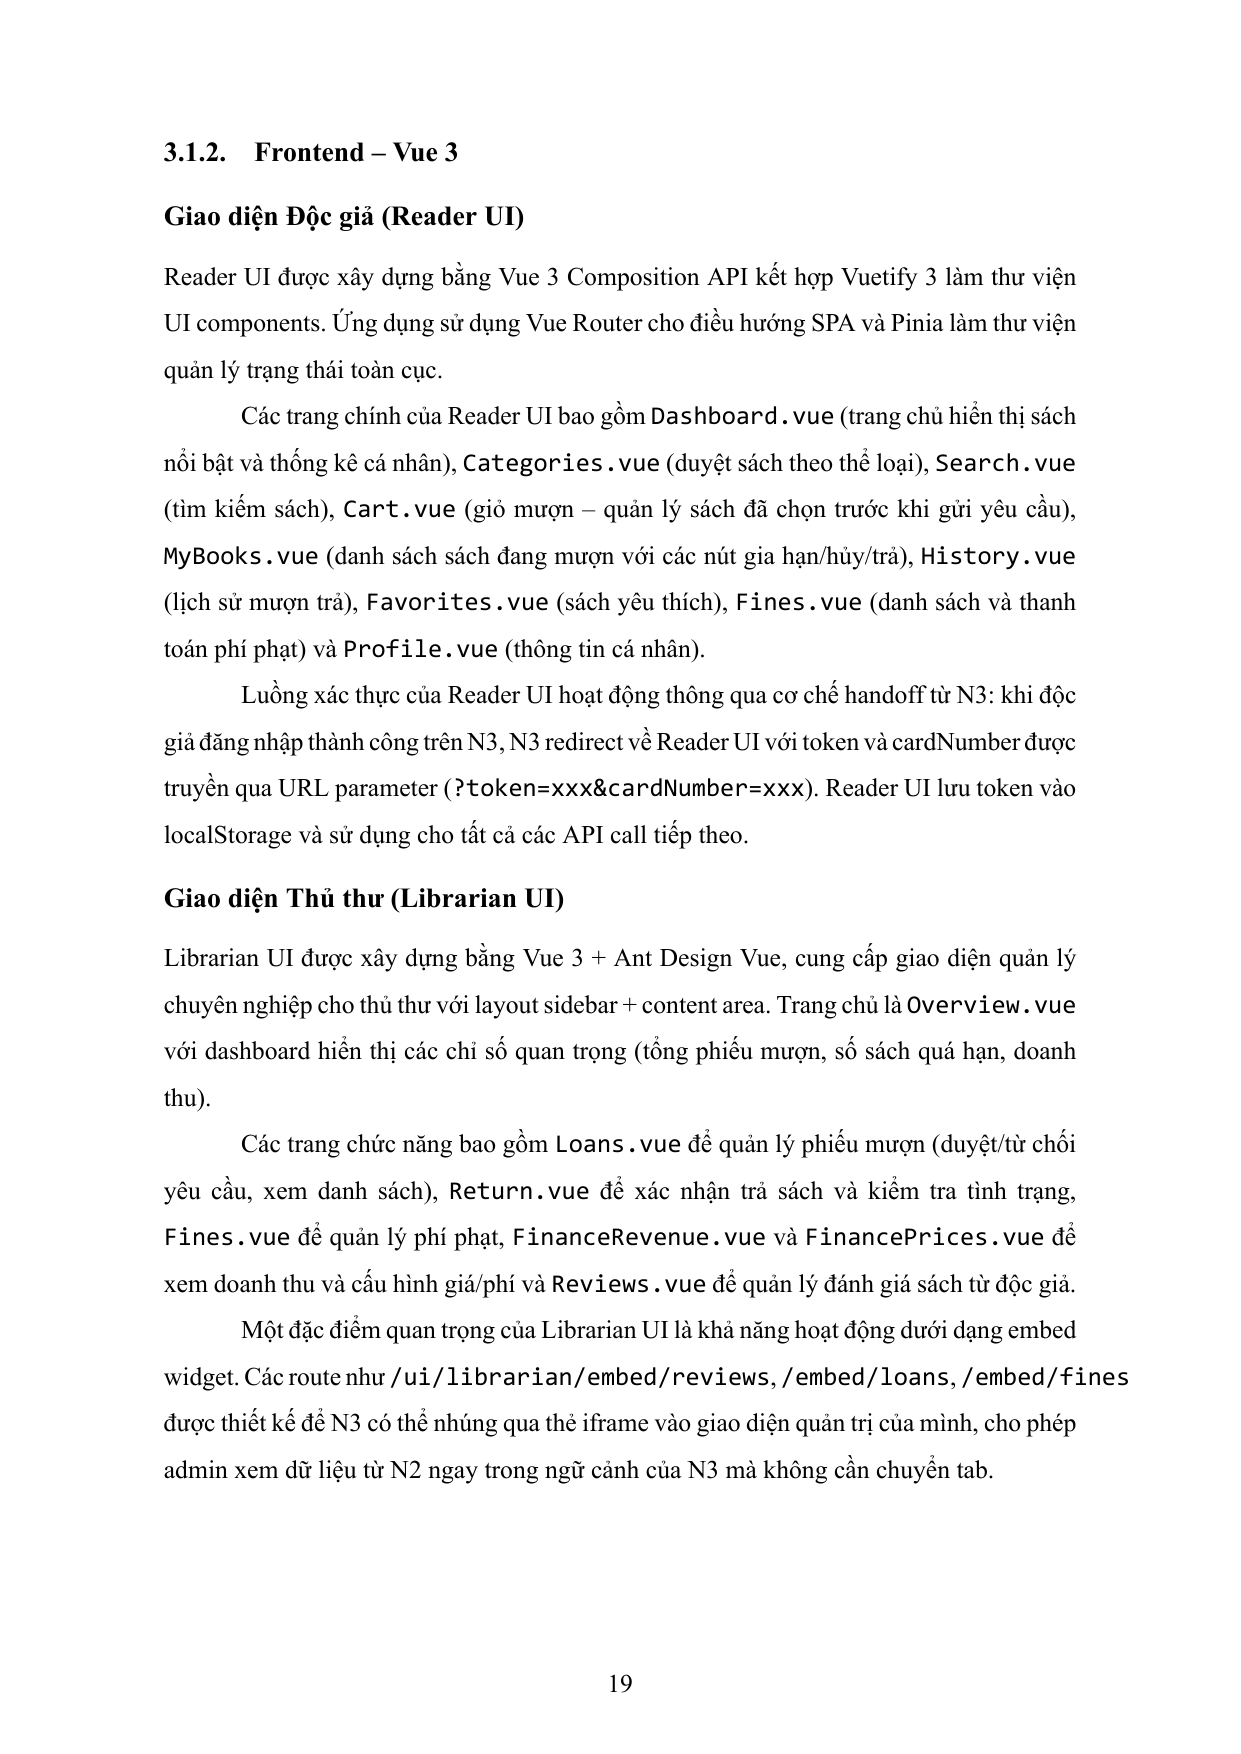
\includegraphics[width=0.98\textwidth]{figures/fig-32-32.png}
\caption{H?nh ?nh/s? ?? tr?ch t? b?o c?o g?c, trang 32}
\end{figure}
\clearpage
\begin{figure}[H]
\centering
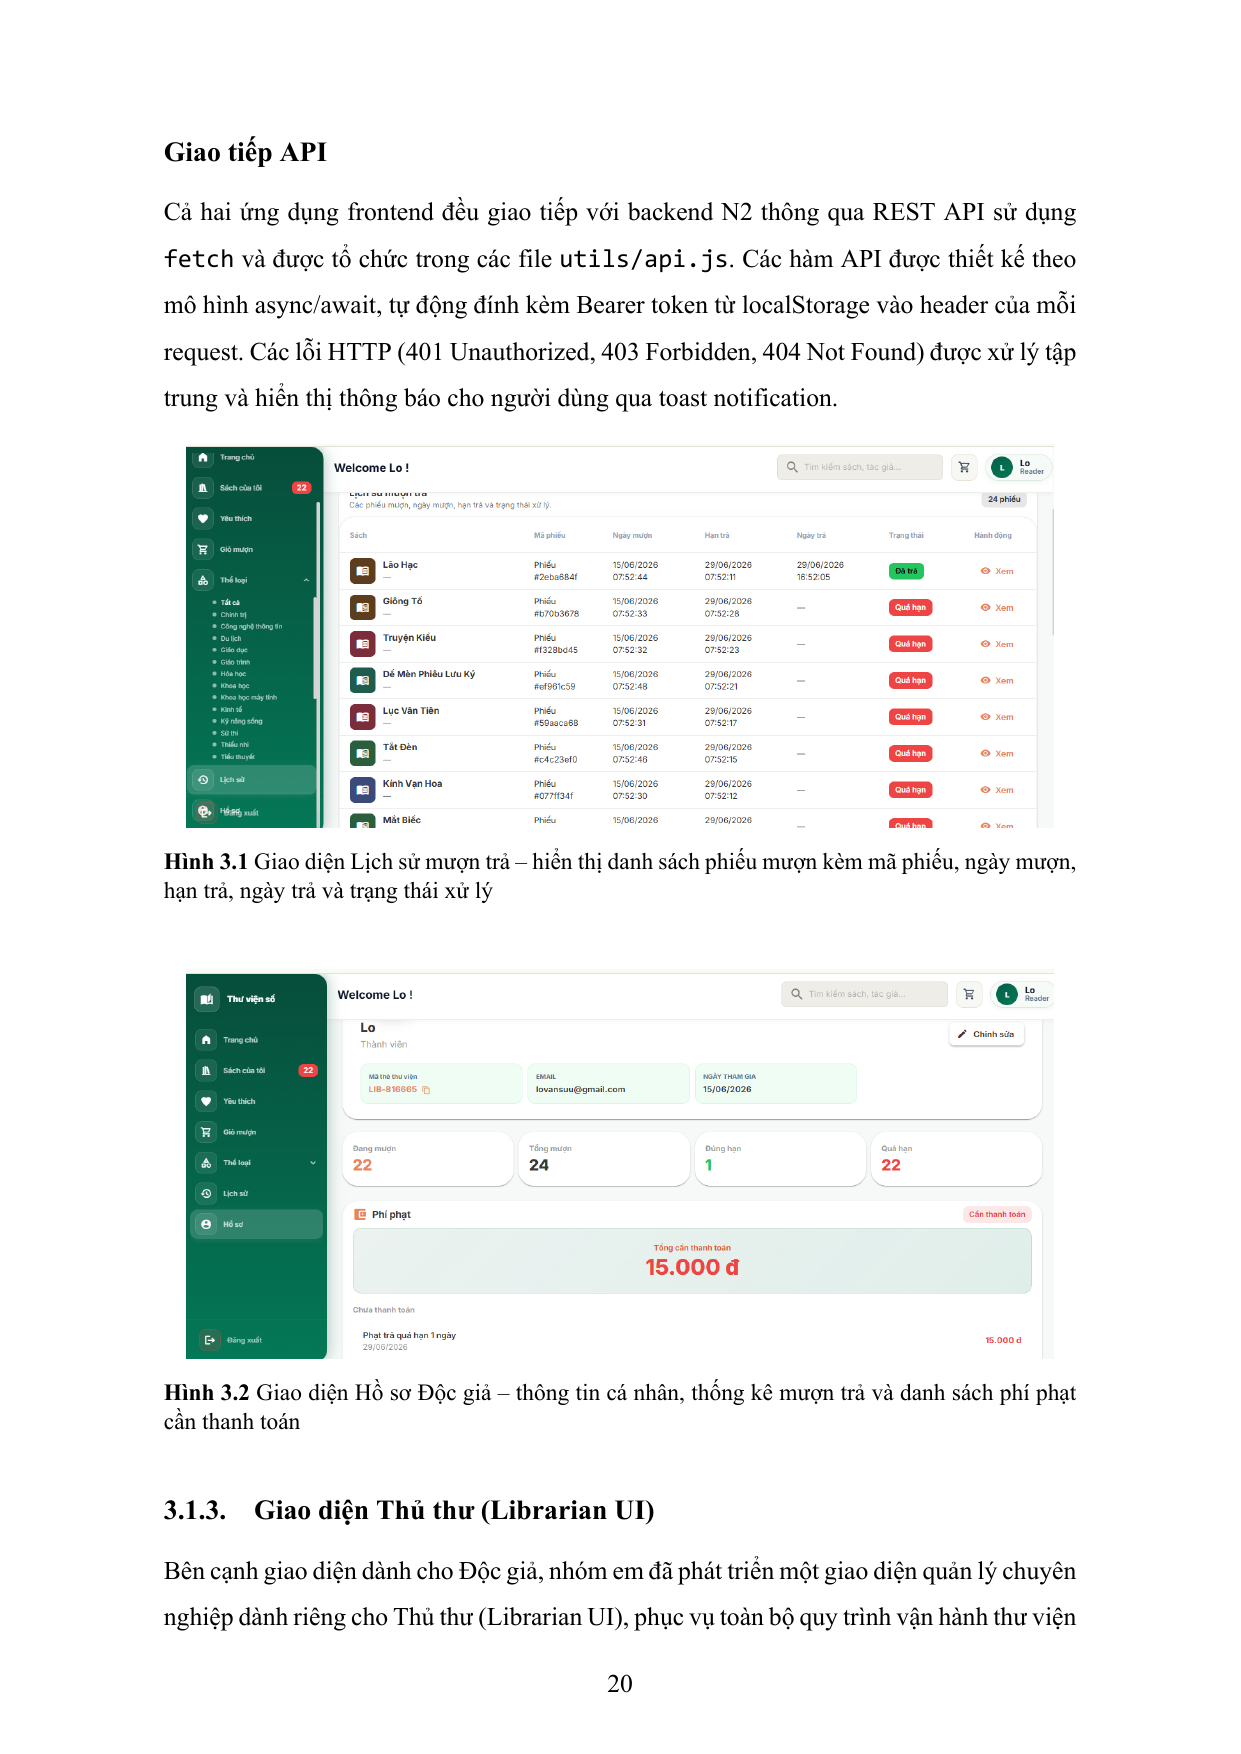
\includegraphics[width=0.98\textwidth]{figures/fig-33-33.png}
\caption{H?nh ?nh/s? ?? tr?ch t? b?o c?o g?c, trang 33}
\end{figure}
\clearpage
\begin{figure}[H]
\centering
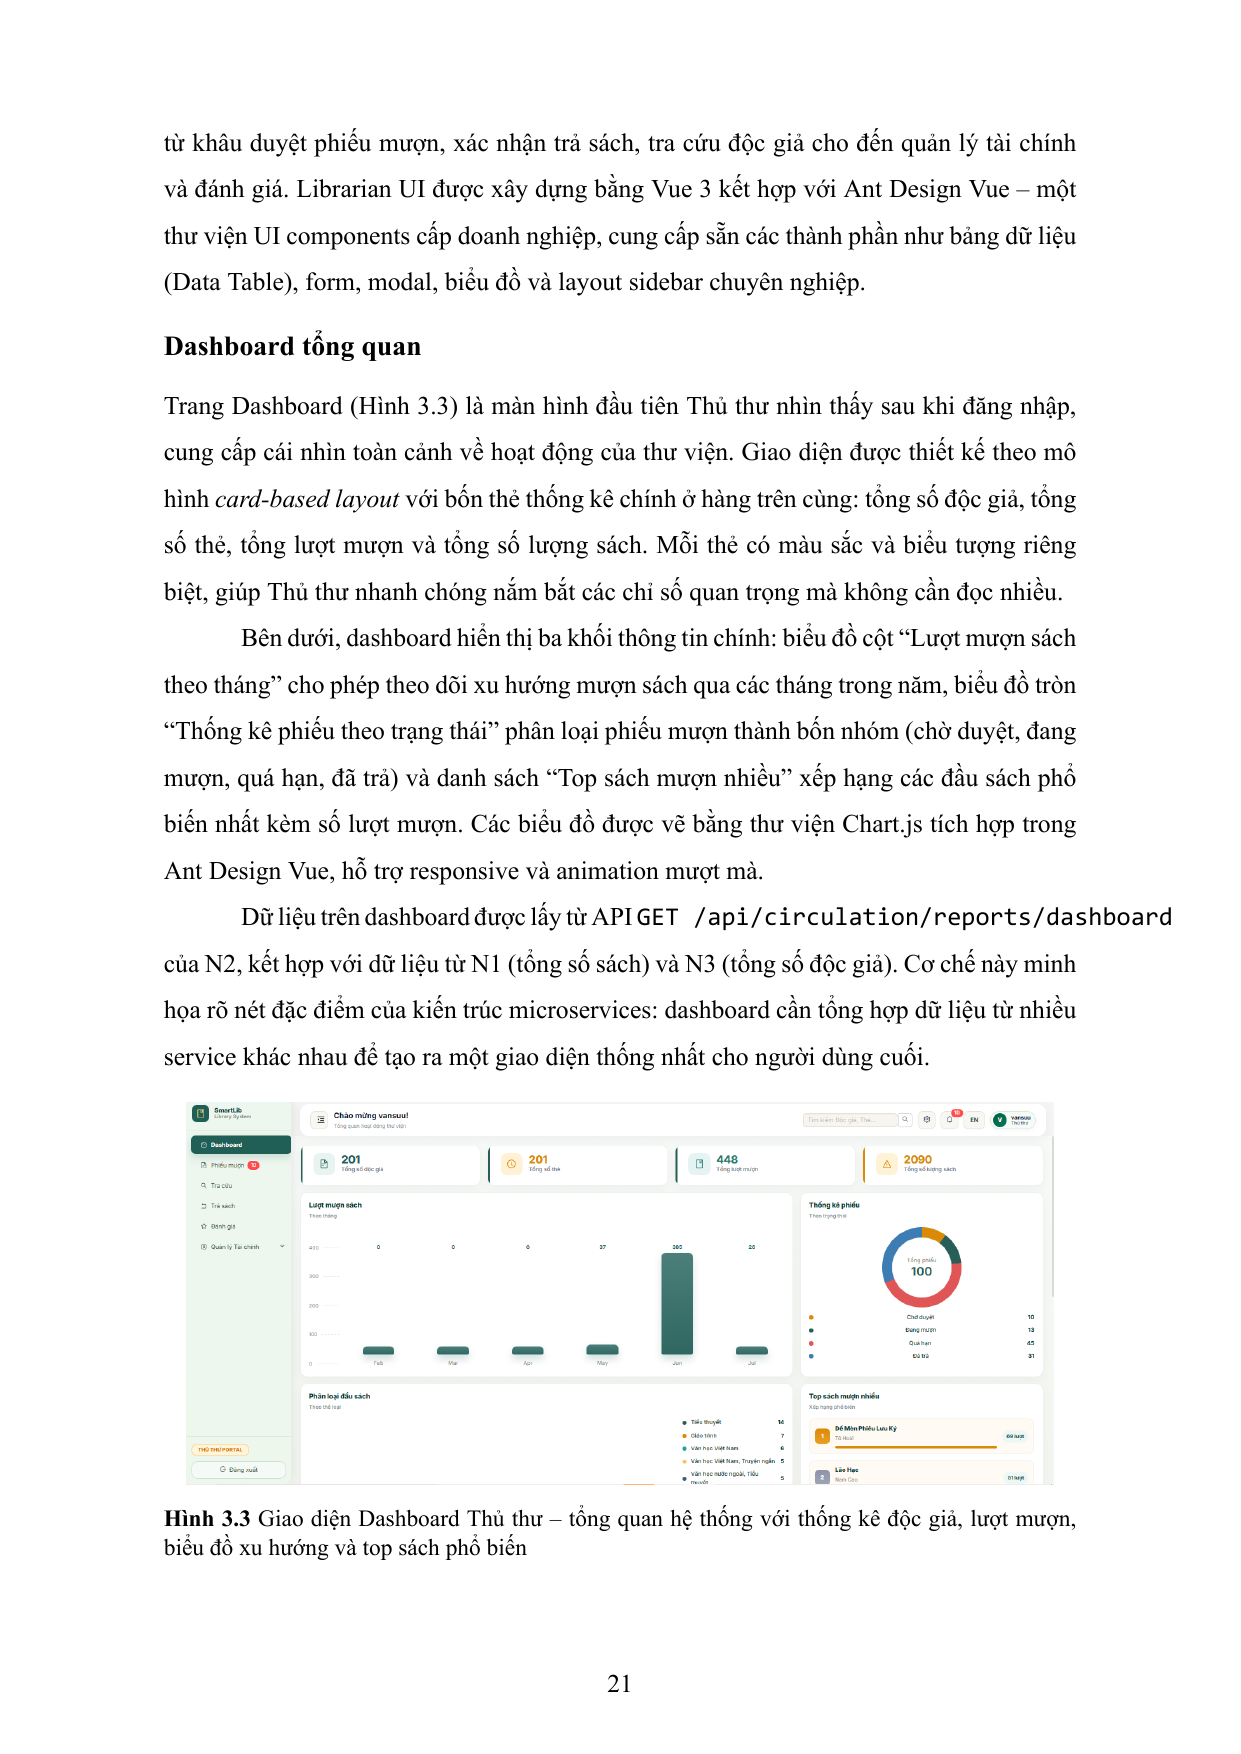
\includegraphics[width=0.98\textwidth]{figures/fig-34-34.png}
\caption{H?nh ?nh/s? ?? tr?ch t? b?o c?o g?c, trang 34}
\end{figure}
\clearpage
\begin{figure}[H]
\centering
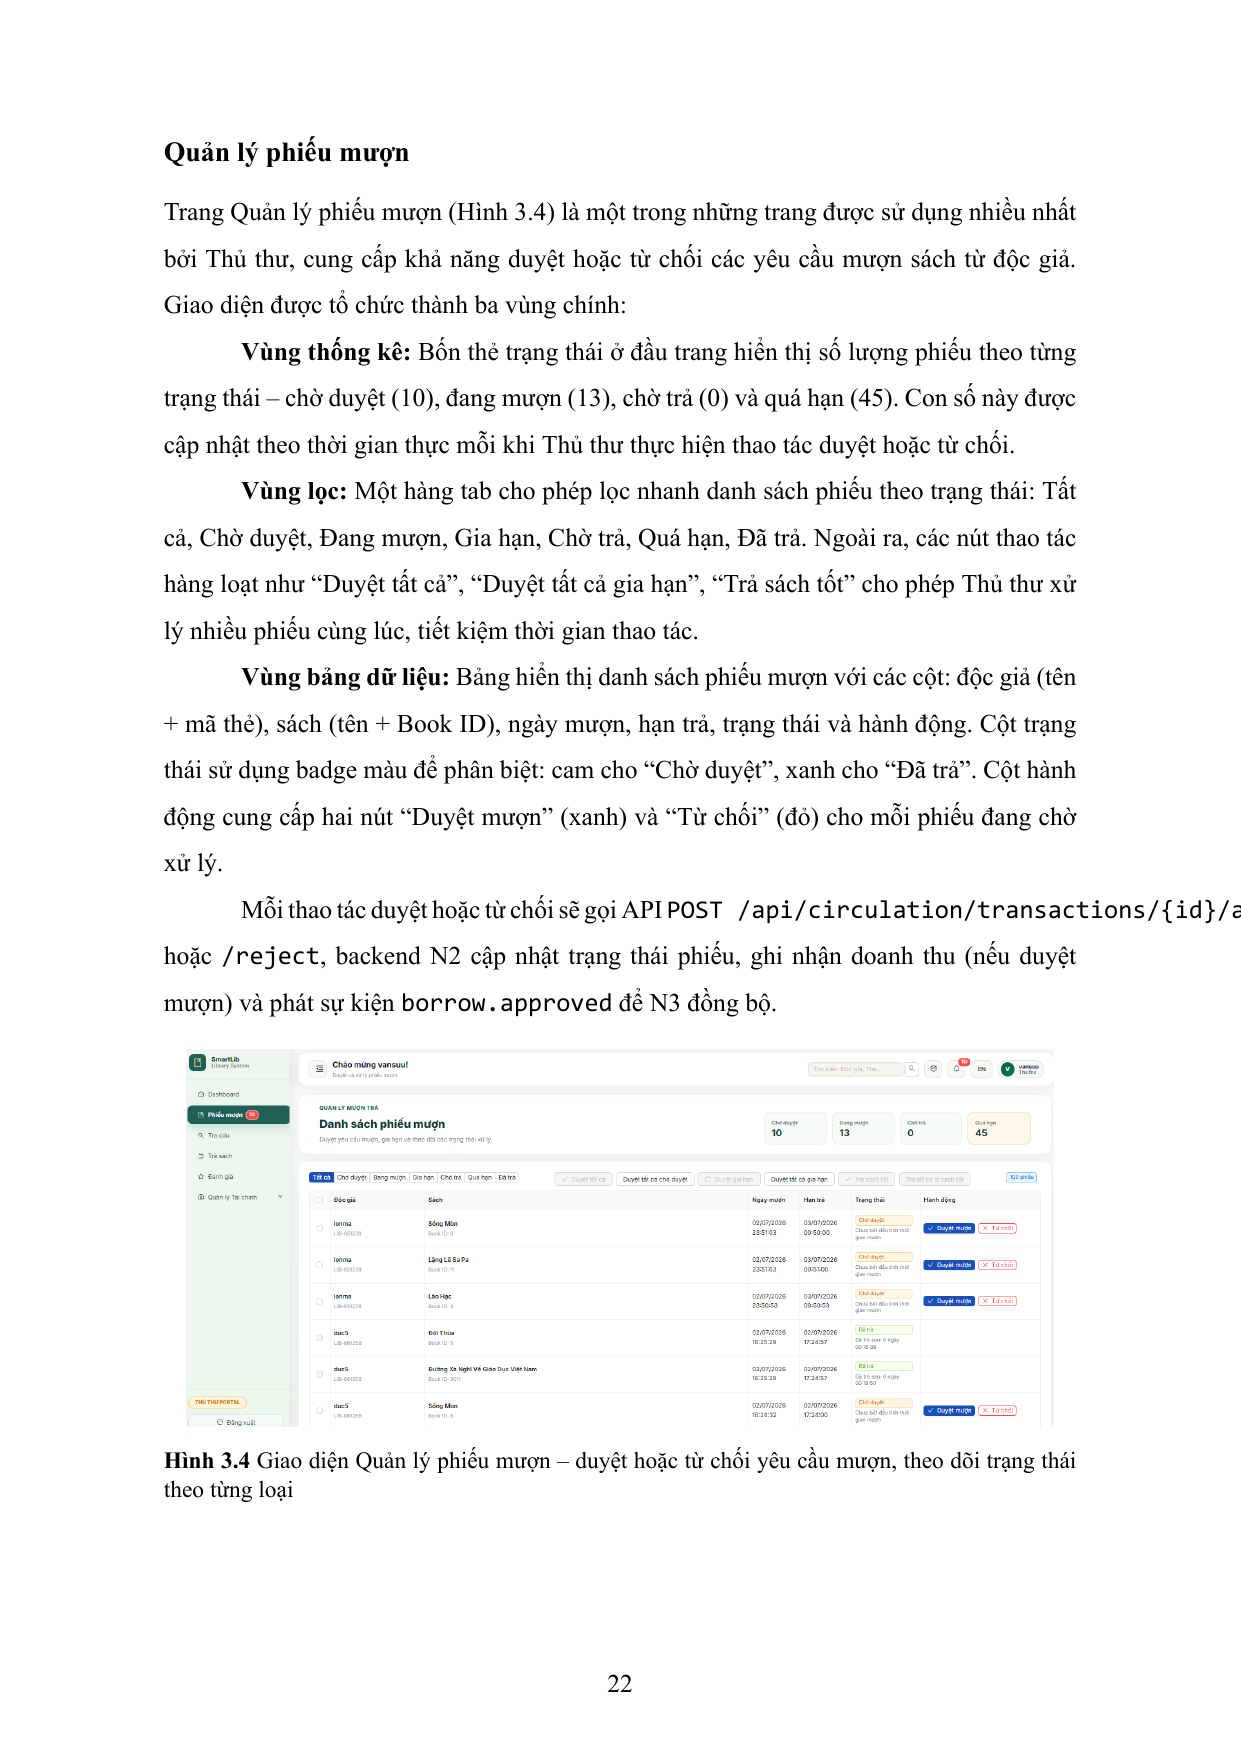
\includegraphics[width=0.98\textwidth]{figures/fig-35-35.png}
\caption{H?nh ?nh/s? ?? tr?ch t? b?o c?o g?c, trang 35}
\end{figure}
\clearpage
\begin{figure}[H]
\centering
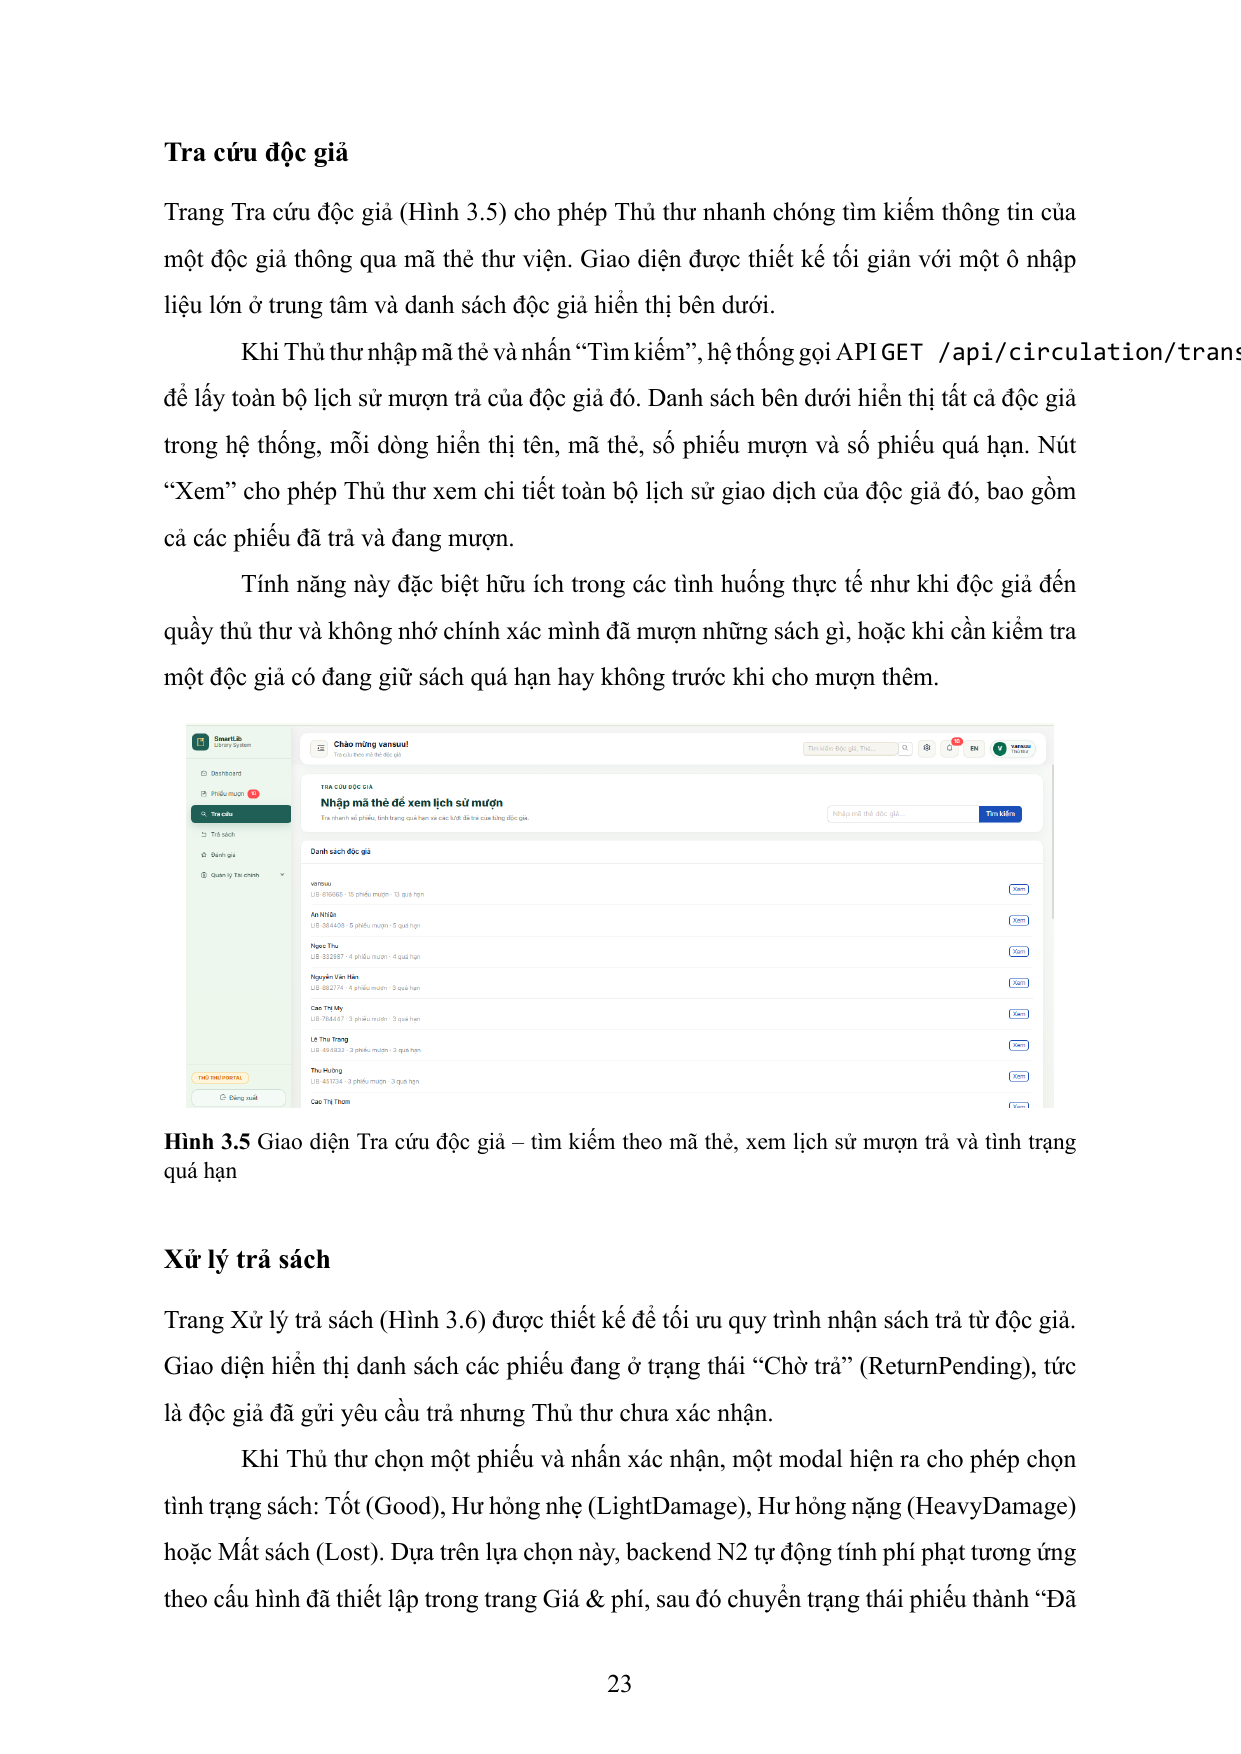
\includegraphics[width=0.98\textwidth]{figures/fig-36-36.png}
\caption{H?nh ?nh/s? ?? tr?ch t? b?o c?o g?c, trang 36}
\end{figure}
\clearpage
\begin{figure}[H]
\centering
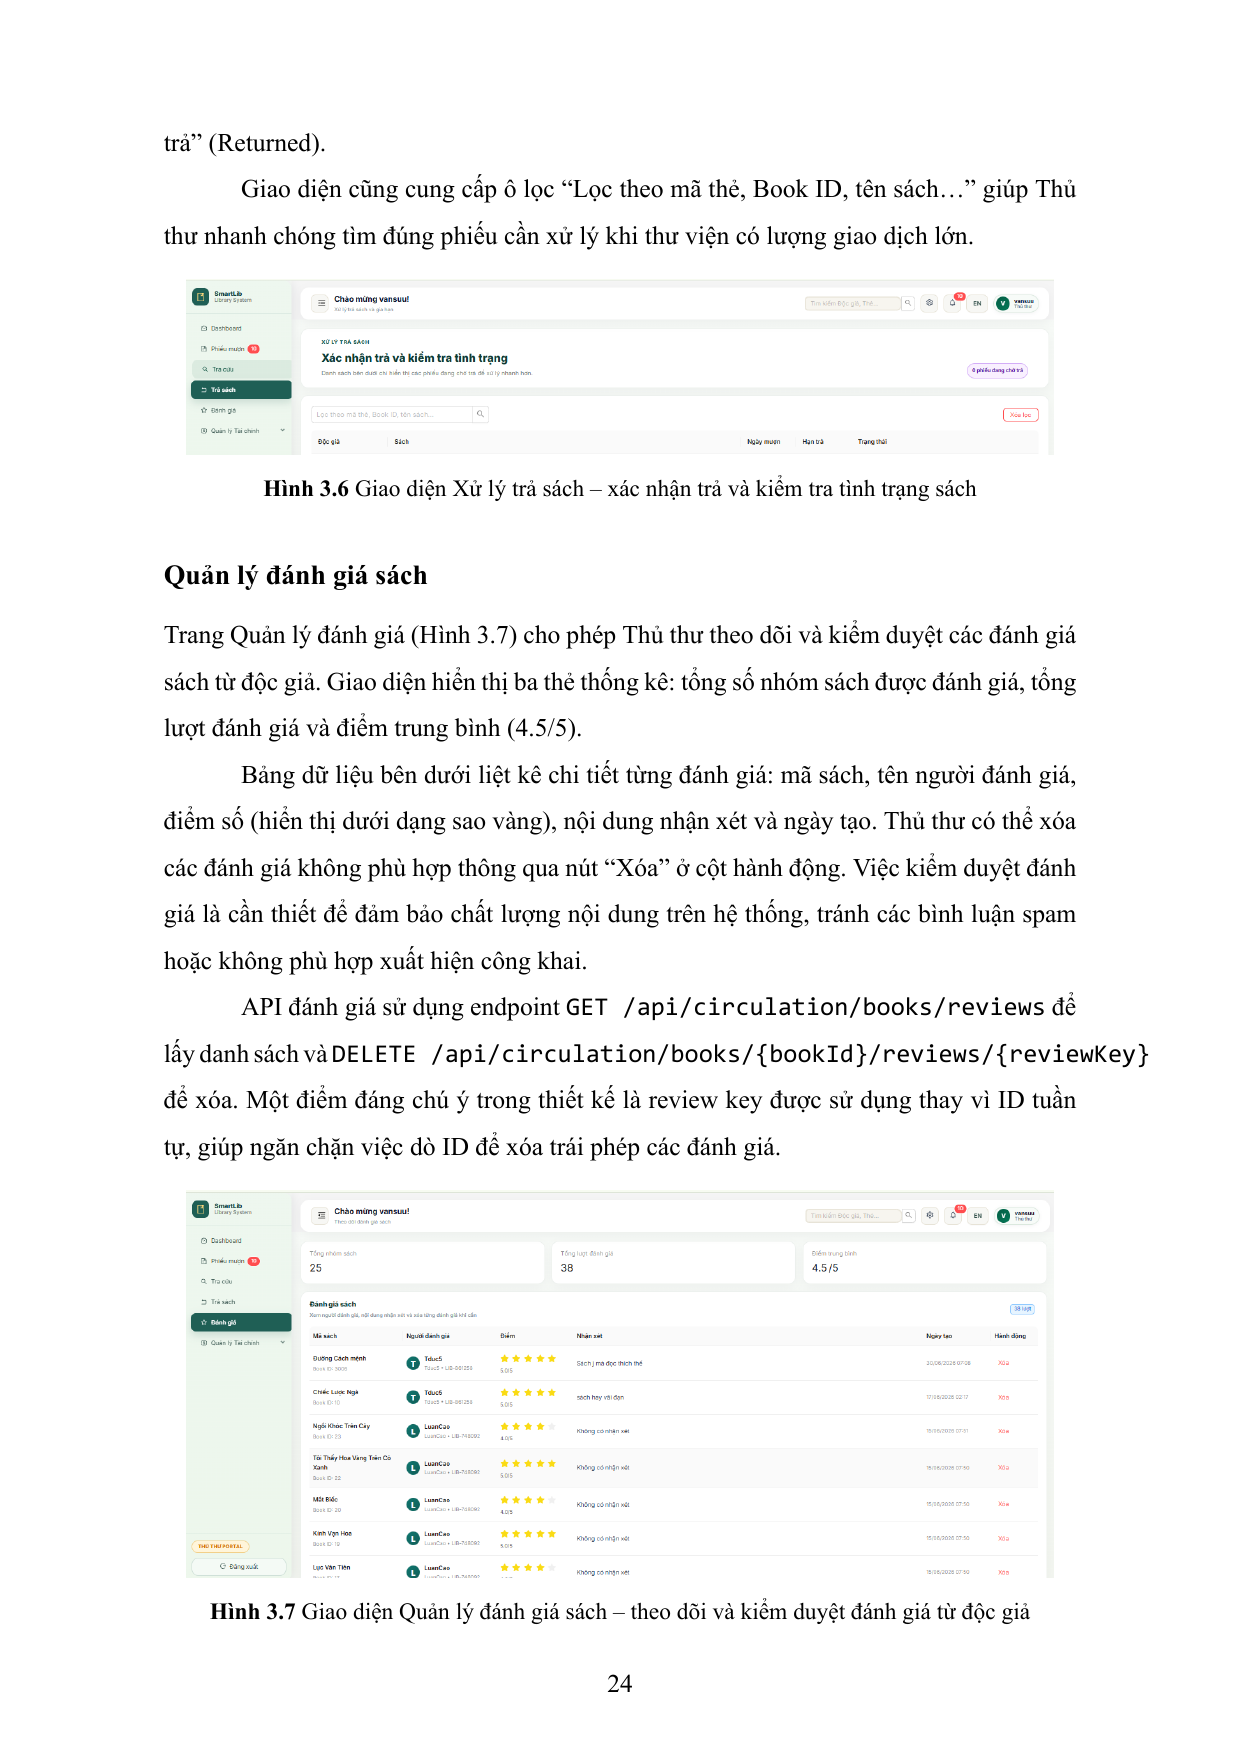
\includegraphics[width=0.98\textwidth]{figures/fig-37-37.png}
\caption{H?nh ?nh/s? ?? tr?ch t? b?o c?o g?c, trang 37}
\end{figure}
\clearpage
\begin{figure}[H]
\centering
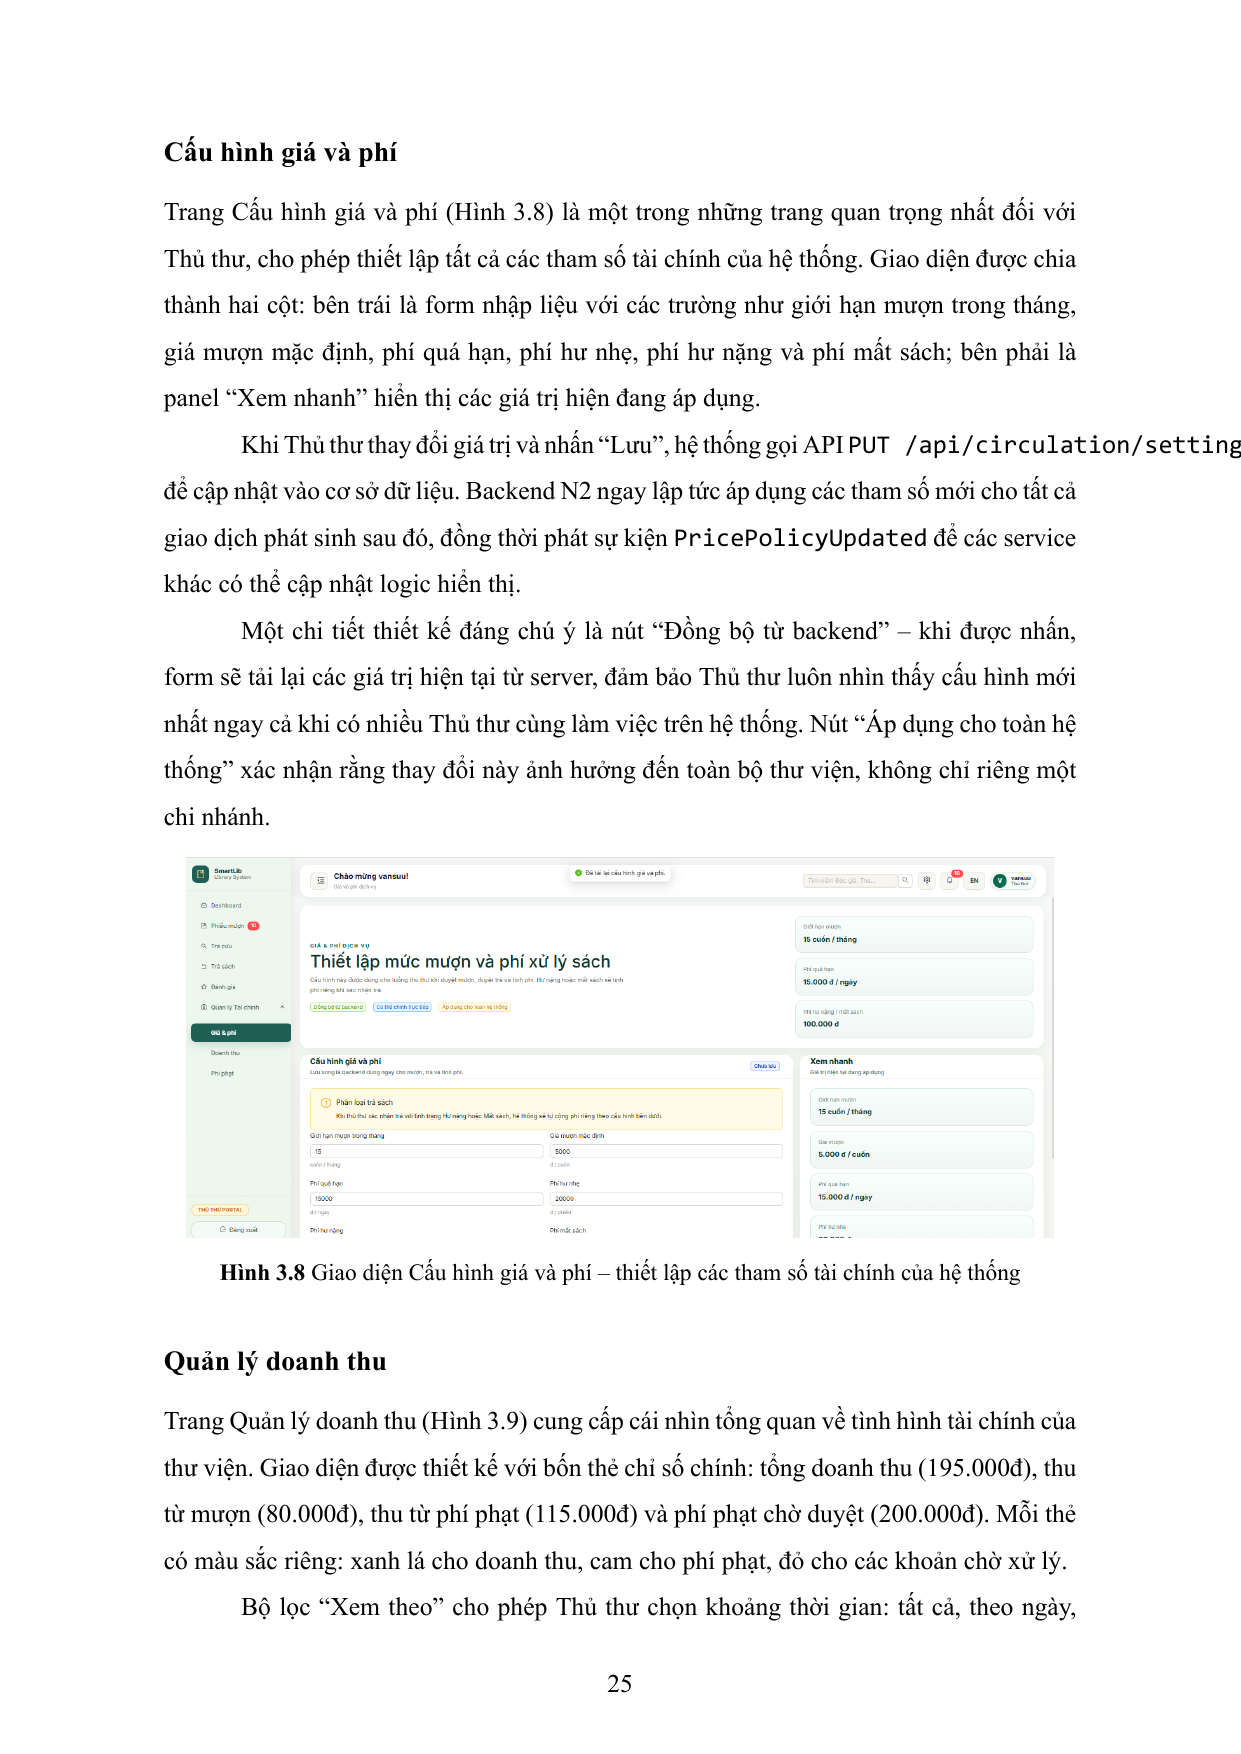
\includegraphics[width=0.98\textwidth]{figures/fig-38-38.png}
\caption{H?nh ?nh/s? ?? tr?ch t? b?o c?o g?c, trang 38}
\end{figure}
\clearpage
\begin{figure}[H]
\centering
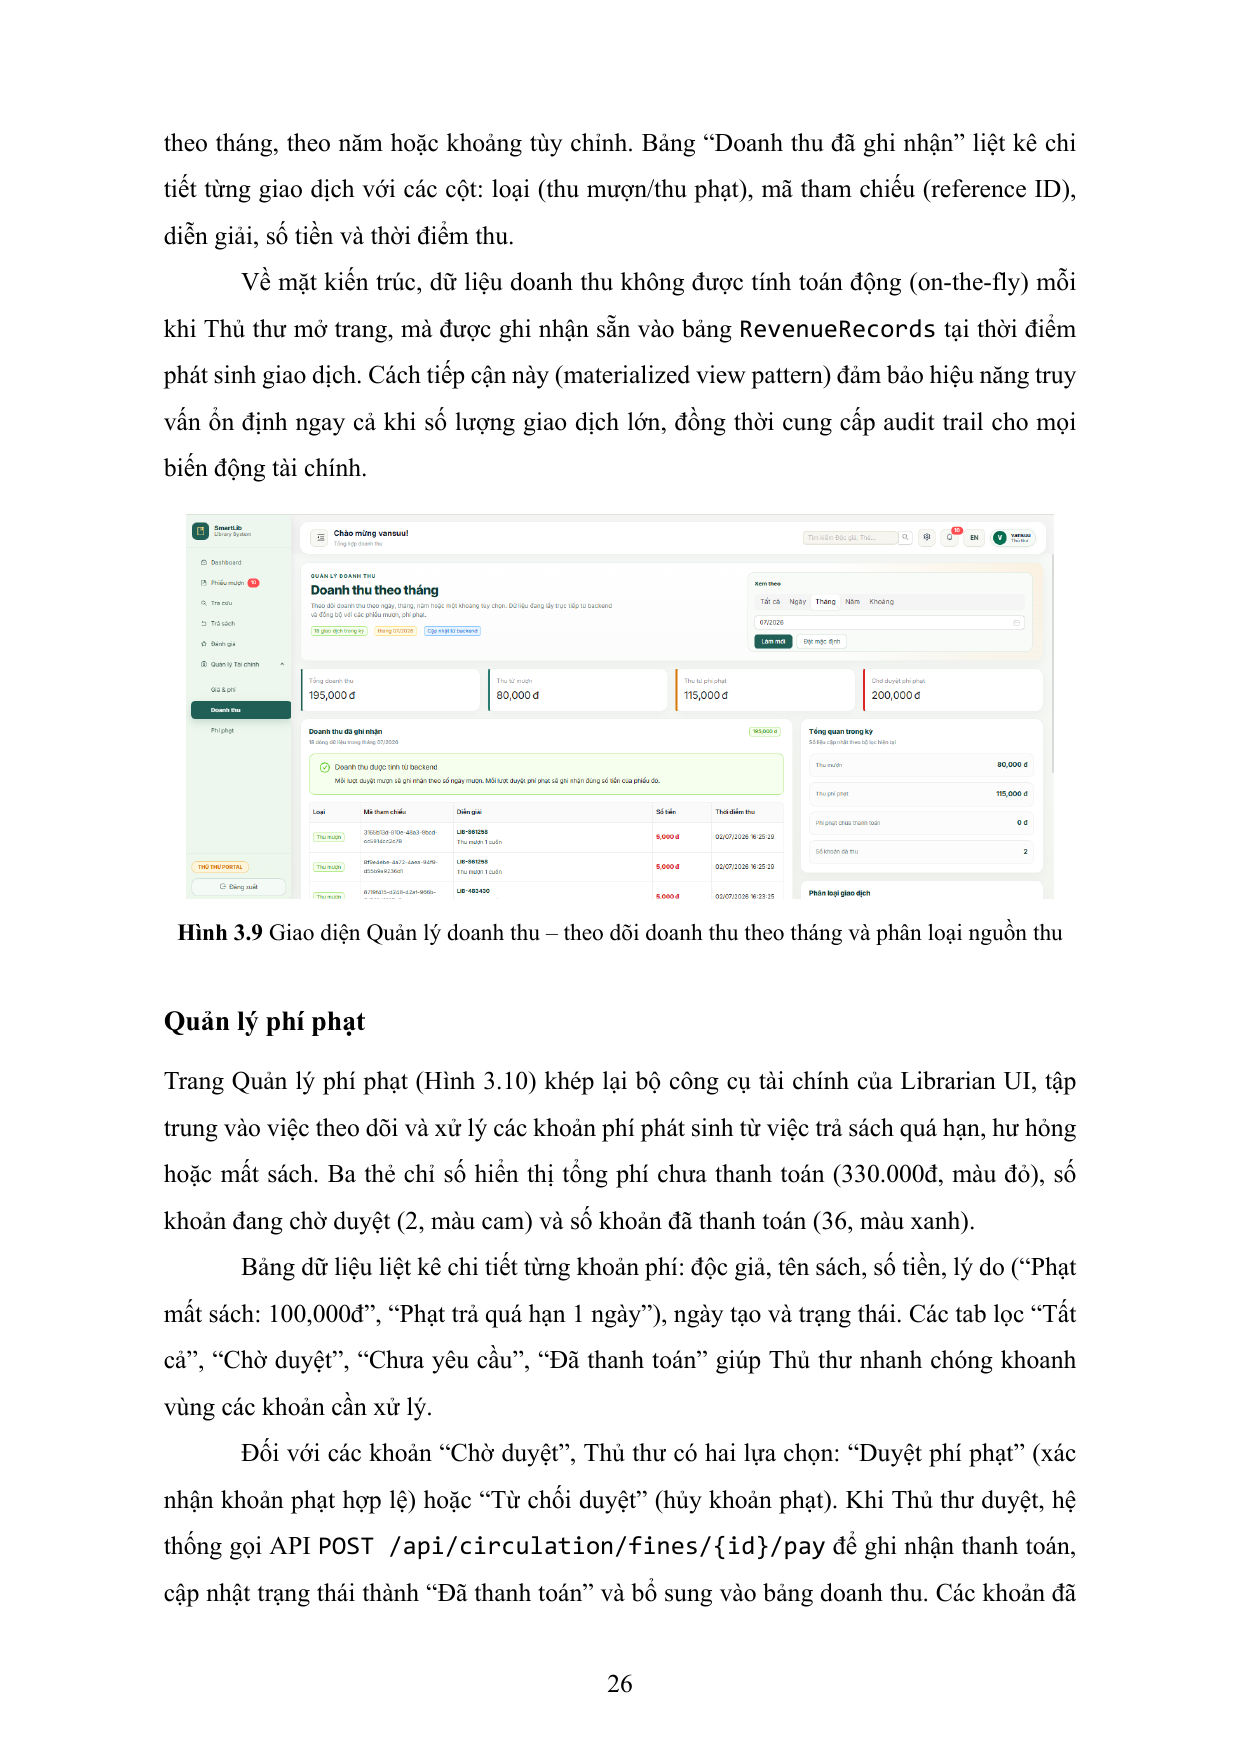
\includegraphics[width=0.98\textwidth]{figures/fig-39-39.png}
\caption{H?nh ?nh/s? ?? tr?ch t? b?o c?o g?c, trang 39}
\end{figure}
\clearpage
\begin{figure}[H]
\centering
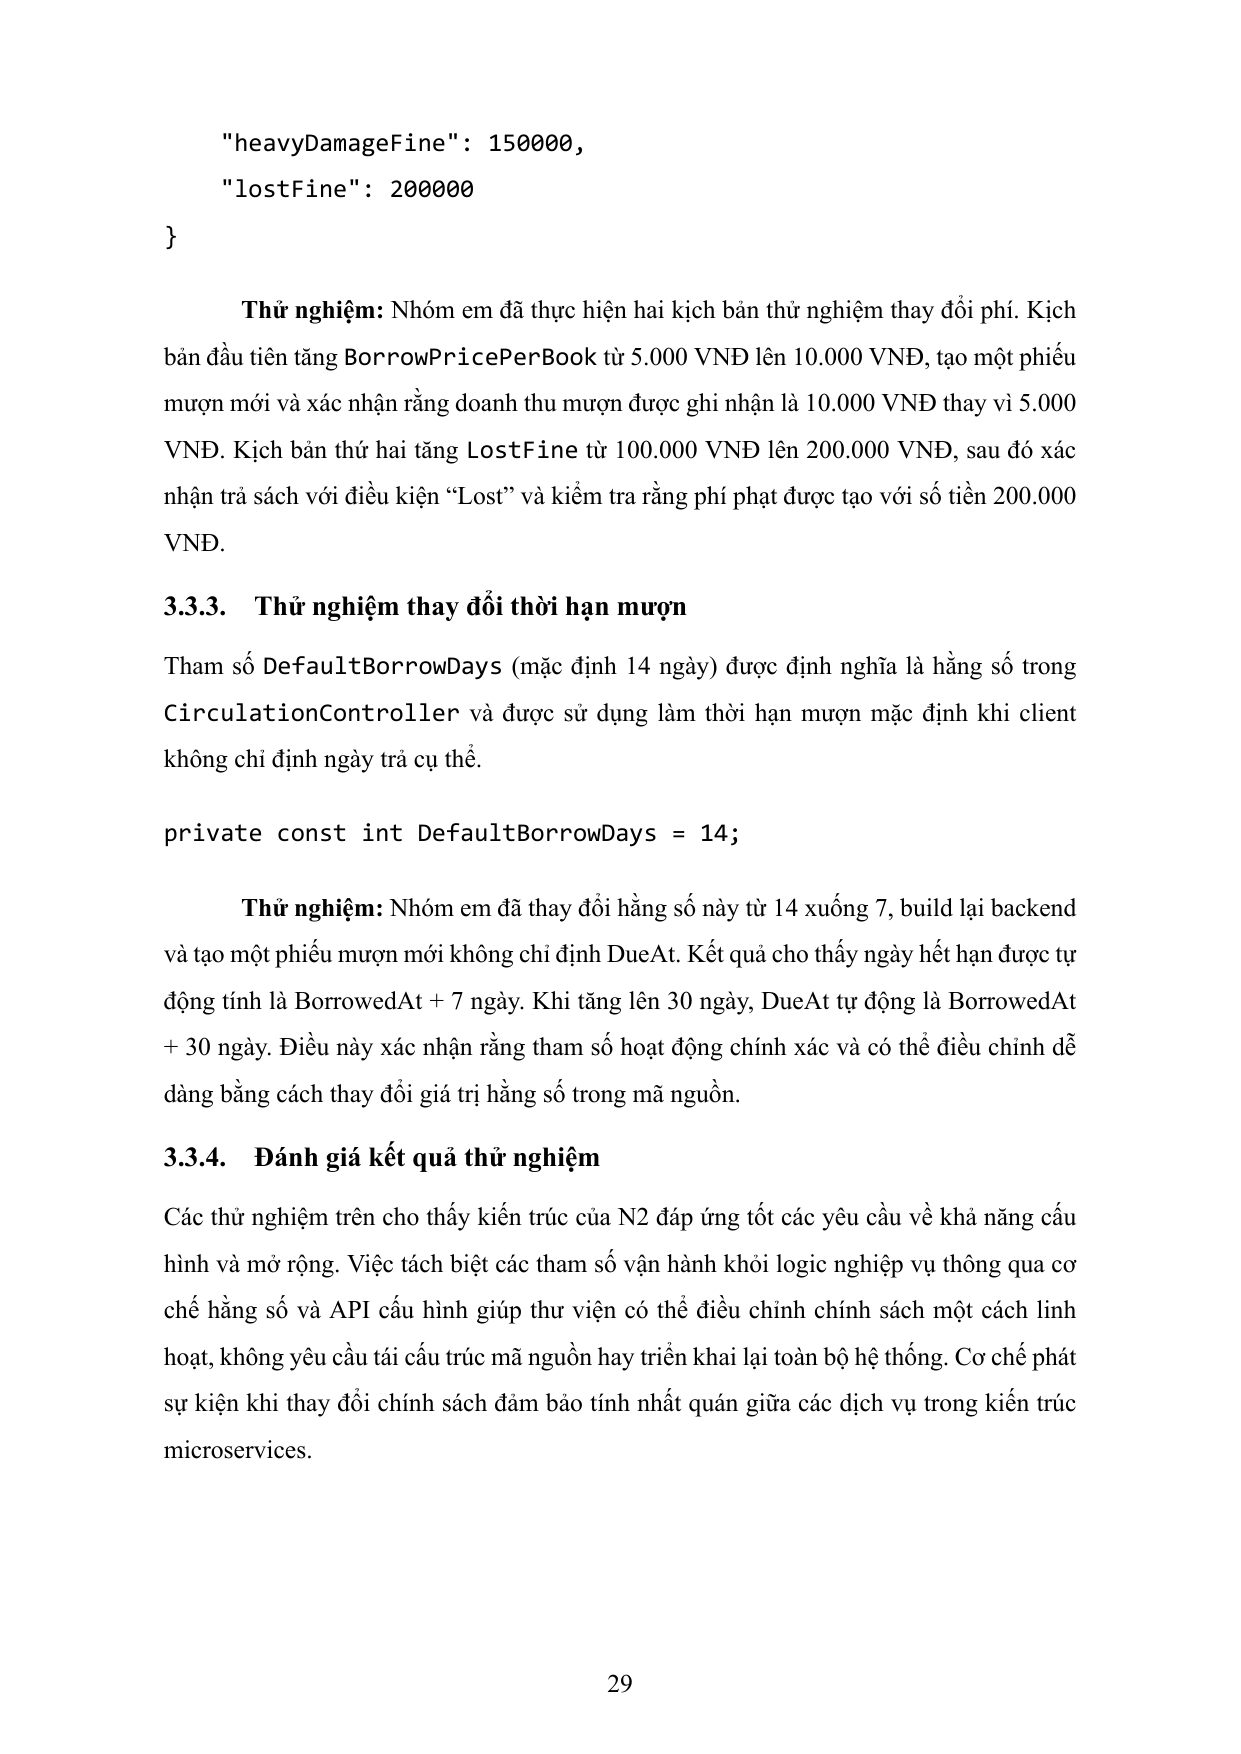
\includegraphics[width=0.98\textwidth]{figures/fig-42-42.png}
\caption{H?nh ?nh/s? ?? tr?ch t? b?o c?o g?c, trang 42}
\end{figure}
\clearpage
\begin{figure}[H]
\centering
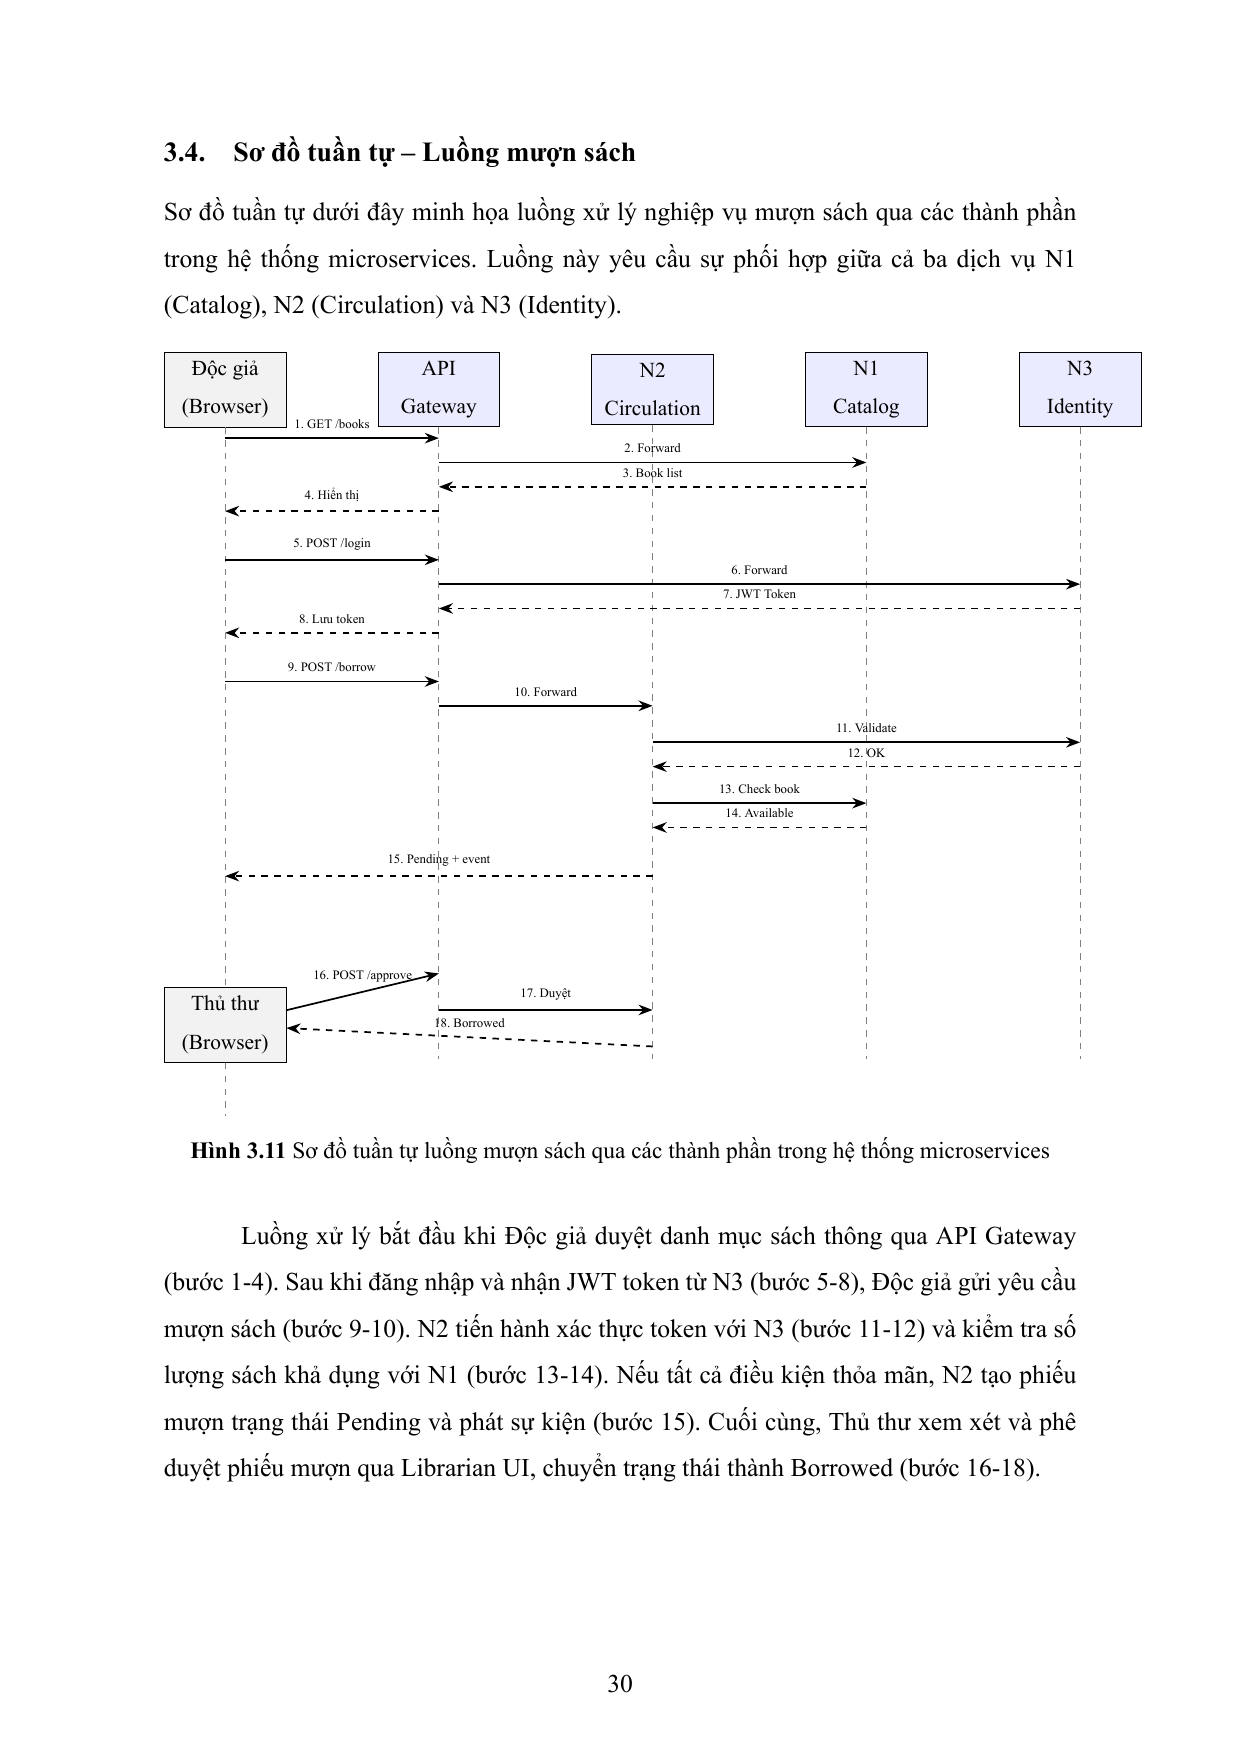
\includegraphics[width=0.98\textwidth]{figures/fig-43-43.png}
\caption{H?nh ?nh/s? ?? tr?ch t? b?o c?o g?c, trang 43}
\end{figure}
\clearpage
